\documentclass{article}

% \usepackage{corl_2020} % Use this for the initial submission.
\usepackage[final]{corl_2020} % Uncomment for the camera-ready ``final'' version.

% IEEE
% \documentclass[letterpaper, 10 pt, conference]{ieeeconf}  % Comment this line out if you need a4paper
%
% \IEEEoverridecommandlockouts                             
% \overrideIEEEmargins

\usepackage[utf8]{inputenc}
\usepackage[T1]{fontenc}
\usepackage{graphicx}
\usepackage{float}
\usepackage{xcolor}
\usepackage[normalem]{ulem}
\usepackage{subfig}

\usepackage{amsmath}
\usepackage{amsfonts}
\usepackage{amssymb}
\usepackage{mathtools}
\usepackage{todonotes}
\usepackage{enumitem}
\usepackage{multicol}
\usepackage{comment}
% \usepackage[noend]{algpseudocode} % this breaks my algorithm box

\usepackage{tikzpagenodes}

% \usepackage[
%   subtle
%   %moderate
% ]{savetrees}

\usepackage{algorithm,algorithmic}

\newcommand{\ph}[1]{{\textbf{#1}:}} % paragraph header
% \newcommand{\todo}[1]{{\color{red} #1 }} % Tasks to do
\newcommand{\note}[1]{{\color{cyan} NOTE: #1 }}
\newcommand{\hn}[1]{{\color{orange} NOTE: (Henry) #1 }}
\newcommand{\gautam}[1]{{\color{cyan}Gautam: #1 }}
% \newcommand{\gautam}[1]{{\color{cyan}}}
\newcommand{\argmax}{\mathop{\mathrm{argmax}}}
\newcommand{\argmin}{\mathop{\mathrm{argmin}}}

\newcommand{\ali}[1]{{\color{blue} #1 }}
%\newcommand{\ali}[1]{} % to remove Ali's comments



\title{
PLGRIM: Hierarchical Value Learning for Large-scale Coverage in Unknown Environments
}
% Keyword: Large-scale, exploration (coverage in unknown environment)


% The \author macro works with any number of authors. There are two
% commands used to separate the names and addresses of multiple
% authors: \And and \AND.
%
% Using \And between authors leaves it to LaTeX to determine where to
% break the lines. Using \AND forces a line break at that point. So,
% if LaTeX puts 3 of 4 authors names on the first line, and the last
% on the second line, try using \AND instead of \And before the third
% author name.

% NOTE: authors will be visible only in the camera-ready (ie, when using the option 'final'). 
% 	For the initial submission the authors will be anonymized.

\author{
  Sung-Kyun Kim*\\
  NASA Jet Propulsion Laboratory\\
  California Institute of Technology\\
  United States\\
  \texttt{sung.kim@jpl.nasa.gov} \\
  \And
  Amanda Bouman*\\
  Department of Mechanical and Civil Engineering\\
  California Institute of Technology\\
  United States\\
  \texttt{abouman@caltech.edu} \\
  \And
  Gautam Salhotra\\
  Department of Computer Science\\
  University of Southern California\\
  United States\\
  \texttt{salhotra@usc.edu} \\
  \And
  David D. Fan\\
  NASA Jet Propulsion Laboratory\\
  California Institute of Technology\\
  United States\\
  \texttt{david.d.fan@jpl.nasa.gov} \\
  \And
  Kyohei Otsu\\
  NASA Jet Propulsion Laboratory\\
  California Institute of Technology\\
  United States\\
  \texttt{kyohei.otsu@jpl.nasa.gov} \\
  \And
  Joel Burdick\\
  Department of Mechanical and Civil Engineering\\
  California Institute of Technology\\
  United States\\
  \texttt{jwb@robotics.caltech.edu} \\
  \And
  Ali-akbar Agha-mohammadi\\
  NASA Jet Propulsion Laboratory\\
  California Institute of Technology\\
  United States\\
  \texttt{aliagha@jpl.nasa.gov} \\
}


\begin{document}
\maketitle

% IEEE
% % \thispagestyle{empty}
% % \pagestyle{empty}
% \pagestyle{plain}

\begin{abstract}
In order for a mobile robot to achieve higher levels of autonomy in previously unexplored environments, it must account for uncertainties in localization, sensor measurements, and unknown hazards, as well as the effect of robot's own actions on these uncertainties. 
%
Making decision in such stochastic setting requires learning value and constructing policies over belief space (space of probability distribution over robot-world state). 
%
Learning value over belief space suffers from computational challenges in large spatial environments (curse of dimensionality) and at long temporal horizons (curse of history) required in many real-world missions. %An effective planner must be computationally efficient and handle time constraints without severely impacting the optimality of the solution.
This work proposes a scalable value learning method over belief space: PLGRIM (Planning at Local-Global levels with Robust Information roadMaps), that bridges the gap between \textit{(i)} local, high-fidelity information such as traversability, and \textit{(ii)} global, macro-level reward seeking behaviors.
%
By leveraging hierarchical belief space planners with information-rich graph structures PLGRIM can address large-scale coverage problems while providing locally near-optimal plans within a receding horizon.
% We take samples of the belief space in order to construct a graph structure that encodes mission and environment-related information, which we call an Information Roadmap (IRM).  
PLGRIM is a step toward enabling belief space planners %aims at bridging the gap between %pushes the boundaries of the state-of-art in 
on physical robots operating in unknown and complex environments. 
%
As a concrete example, we demonstrate the performance of PLGRIM on Boston Dynamics' quadruped SPOT robot operating in unstructured environments.
%and demonstrate its performance as the planning core of the NeBula 2.0 autonomy framework. NeBula 1.0 (prior to PLGRIM integration) framework and the adopted hardware in this demonstration have contributed to winning first place in the 2020 DARPA Subterranean Challenge, Urban Circuit.

%In  particular,  we  will  discuss  the  behaviors  andcapabilities  which  emerge  from  the  integration  of  the  auton-omy  architecture  NeBula  (Networked  Belief-aware  PerceptualAutonomy)   with   next-generation   mobility   systems.   We   willdiscuss  the  hardware  and  software  challenges,  and  solutionsin mobility, perception, autonomy, and wireless networking, aswell  as  lessons  learned  and  future  directions.  

%our framework for autonomous exploration in simulation with large environments with rough terrains and complex topology.
% We demonstrate our framework in team CoSTAR's participation in the DARPA Subterranean Challenge, in which teams compete to autonomously search for artifacts in large, unknown, GPS-denied environments.
% \gautam{Need to update. possible phrases: active learning, online planning, planning under uncertainty, learning value function in POMDP, MCTS, }
\end{abstract}

% \gautam{PLGRIM (pilgrim): Planning at Local and Global levels with Robust Information Maps}

% Two or three meaningful keywords should be added here
% \keywords{Coverage planning under uncertainty, Hierarchical planning, POMDP} 
\keywords{Stochastic coverage, POMDP, Value learning, Hierarchical planning}



% %%%%%%%%%%%%%%%%%%%%%%%%%%%%%%%%%%%%%%%%%%%%%%%%%%%%%%%%%%%%%%%%%%%%%%%%%%%%%%%%
% \section{Instructions}

% \ph{Paragraph header} Please start every single paragraph with a paragraph header, summarizing the intention of that paragraph. This is mainly for iterations during the paper preparation. We will remove most of them for the final report.

% {
% \color{orange}
% For the "notation consistency", please take a look at these works (note that the content might NOT be relevant, but notation could be useful)

% \begin{itemize}
% \item Feedback based IRM (for graph abstraction notation):
% FIRM: Sampling-based Feedback Motion Planning Under Motion Uncertainty and Imperfect Measurements (IJRR 2014)

% https://journals.sagepub.com/doi/10.1177/0278364913501564

% \item For 3D grid mapping with "information encoding"
% https://eric-heiden.com/publication/2019-crm-ijrr/

% \item For risk-aware local planning over confidence rich maps:
% https://eric-heiden.com/publication/2017-crm-to-iros/2017-crm-to-iros.pdf
% \end{itemize}


% }

%%%%%%%%%%%%%%%%%%%%%%%%%%%%%%%%%%%%%%%%%%%%%%%%%%%%%%%%%%%%%%%%%%%%%%%%%%%%%%%%

% Abstract
% 1 Introduction
% 2 Related work
% 3 Problem description/formulation
% -Coverage planning (SubT)
% -POMDP
% 4 Exploration-Coverage Planning Problem
% 5 Overall solution framework
% -Global/local IRM
% -Hierarchical planning
% -System overview
% 6 Algorithm description
% -(POMCP-based coverage planning)
% -Graph-level Planner
% -Lattice-level Planner
% 7 Experimental results
% -Simulation
% -Robot experiments
% 7 Conclusion
% Appendix


%%%%%%%%%%%%%%%%%%%%%%%%%%%%%%%%%%%%%%%%%%%%%%%%%%%%%%%%%%%%%%%%%%%%%%%%%%%%%%%%
\section{Introduction}

%\ph{High-level mission}
Consider a large-scale coverage mission in an unknown environment, in which a robot is tasked with exploring and searching a GPS-denied unknown area, under given time constraints. Essential elements of an autonomy architecture needed to realize such a mission include creating a map of the environment, accurately predicting risks, and planning motions that can meet the coverage and time requirements while minimizing risks.  In such an architecture, quantifying and planning over uncertainty is essential for creating robust, intelligent, and optimal behaviors.

From value learning perspective, a coverage planning problem in an unknown space can be considered an active learning problem over the robot's belief, where belief is defined as the probability distributions over all possible joint robot-world states.
%
The objective is to find the best action sequence that maximizes the accumulated reward over time.  The agent must accumulate data to incrementally build a model of its environment, and must understand the effects of its actions on the quality and quantity of data it collects.

%\ph{Problem description--POMDP perspective}
Since the agent's future actions affect its belief of the world and robot state, this coverage problem is fundamentally a Partially Observable Markov Decision Process (POMDP) problem.
%A POMDP is a principled formalization of 
%a sequential decision making process under motion and sensing uncertainty.
The agent employs the underlying intrinsic model of the sequential action-observation process under uncertainty, so that it can %(asymptotically) converge to the optimal solution in a more 
expand its search structure over the space and learn the value in a more sample-efficient manner than model-free learning approaches.



% \begin{figure}[t]
%   \centering
% %   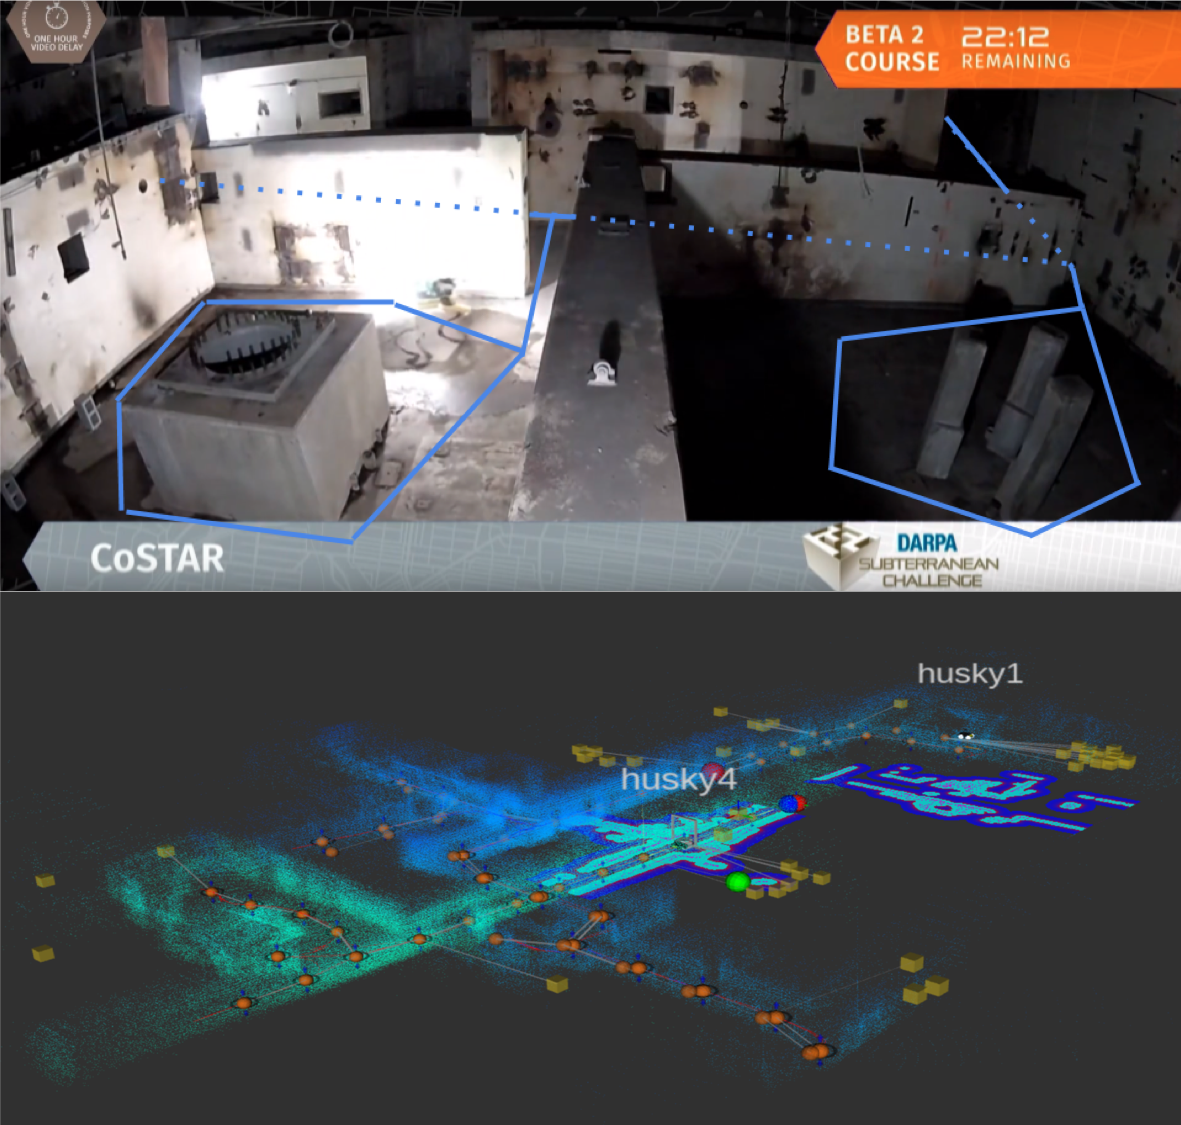
\includegraphics[width=.48\textwidth]{figures/firstpage_v2.png}
%   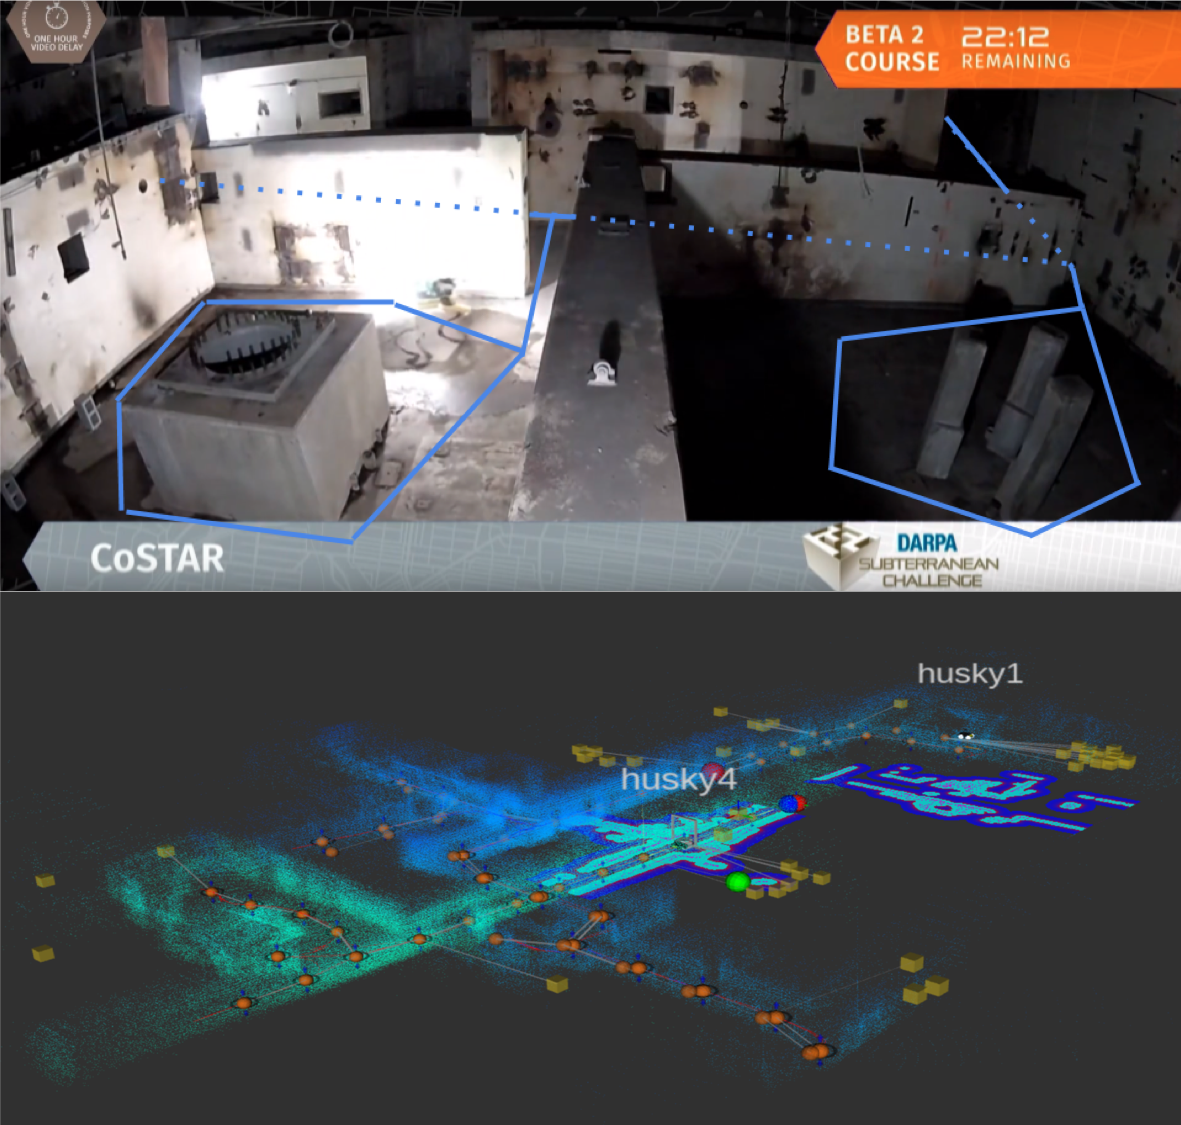
\includegraphics[width=.7\textwidth,trim={0 0 0 11.0cm},clip]{figures/firstpage_v2.png}
%   \caption{ %The top figure shows a portion of the course in the Urban Circuit of the DARPA Subterranean Challenge. The blue line highlights two neighboring rooms joined by a narrow passage. CoSTAR efficiently explored both rooms by planning on the IRM. 
%   IRM and lattice visualization during an autonomous exploration mission.}
%   \label{fig:firstPage}
% \end{figure}

% \begin{figure}[t!]
%   \centering
%   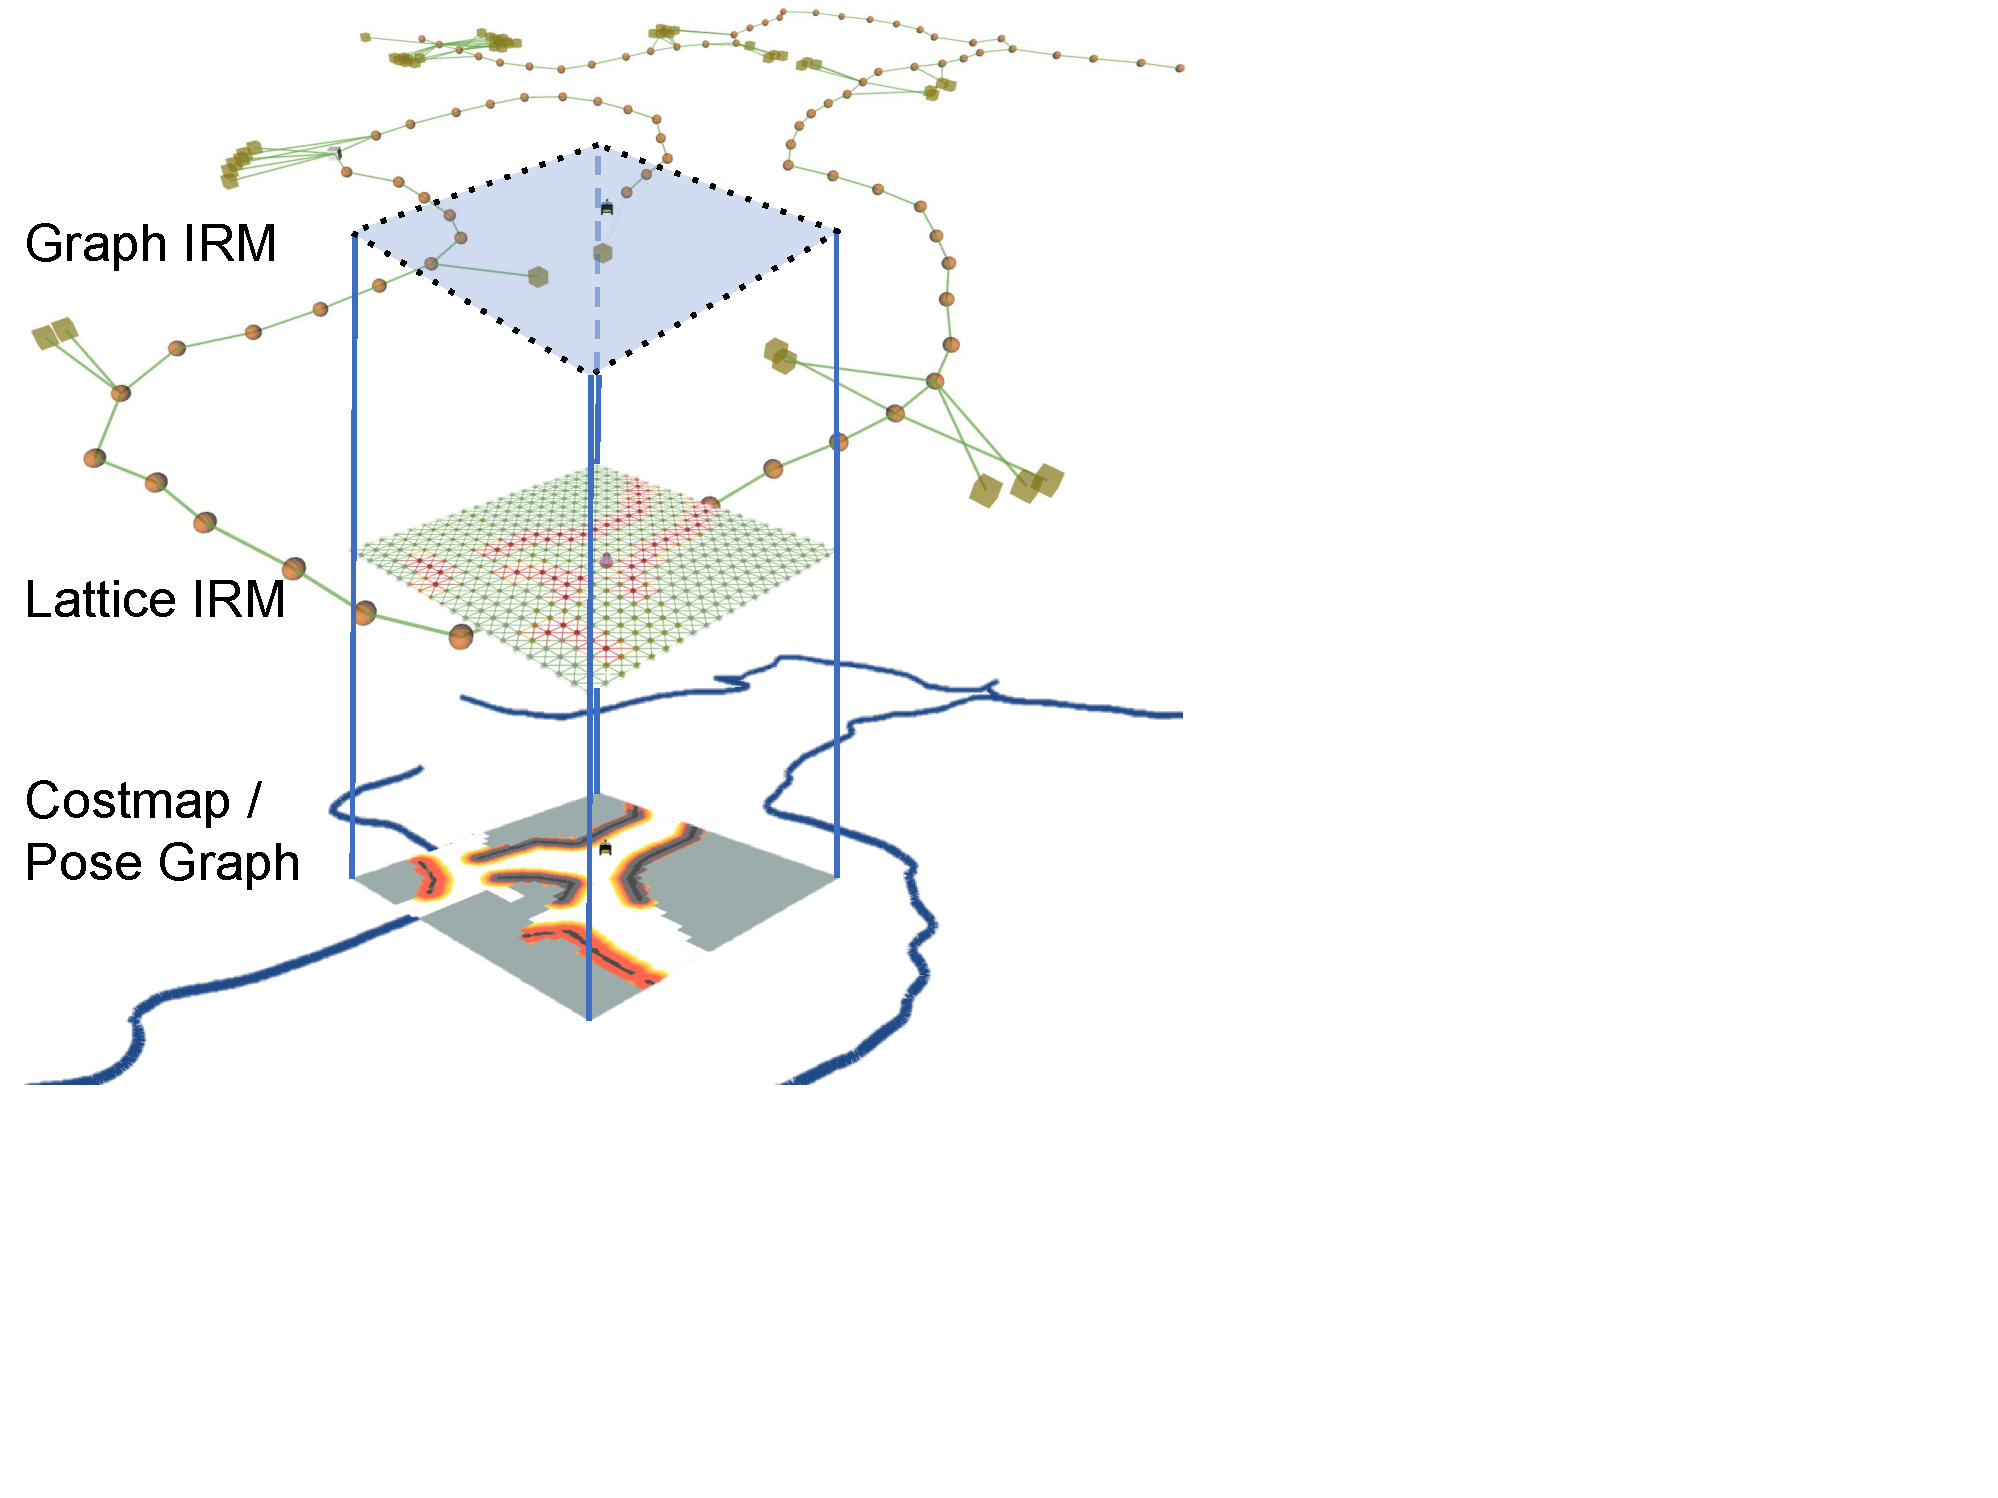
\includegraphics[width=.4\textwidth]{figures/graph-lattice-map.pdf}
%   \caption{Visualization of hierarchical Information RoadMaps (IRMs).}
%   \label{fig:firstPage}
% \end{figure}
% \begin{figure}[t!]
%   \centering
%   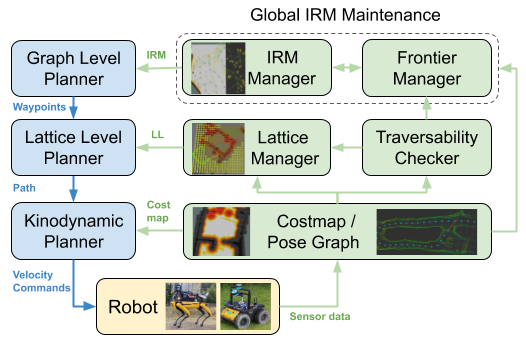
\includegraphics[width=.6\textwidth]{figures/SystemOverview.png}
%   \caption{[WIP] System overview}
%   \label{fig:system_overview}
% \end{figure}
\begin{figure}[ht!]
  \centering
  \subfloat[System diagram\label{fig:system_overview}]{
    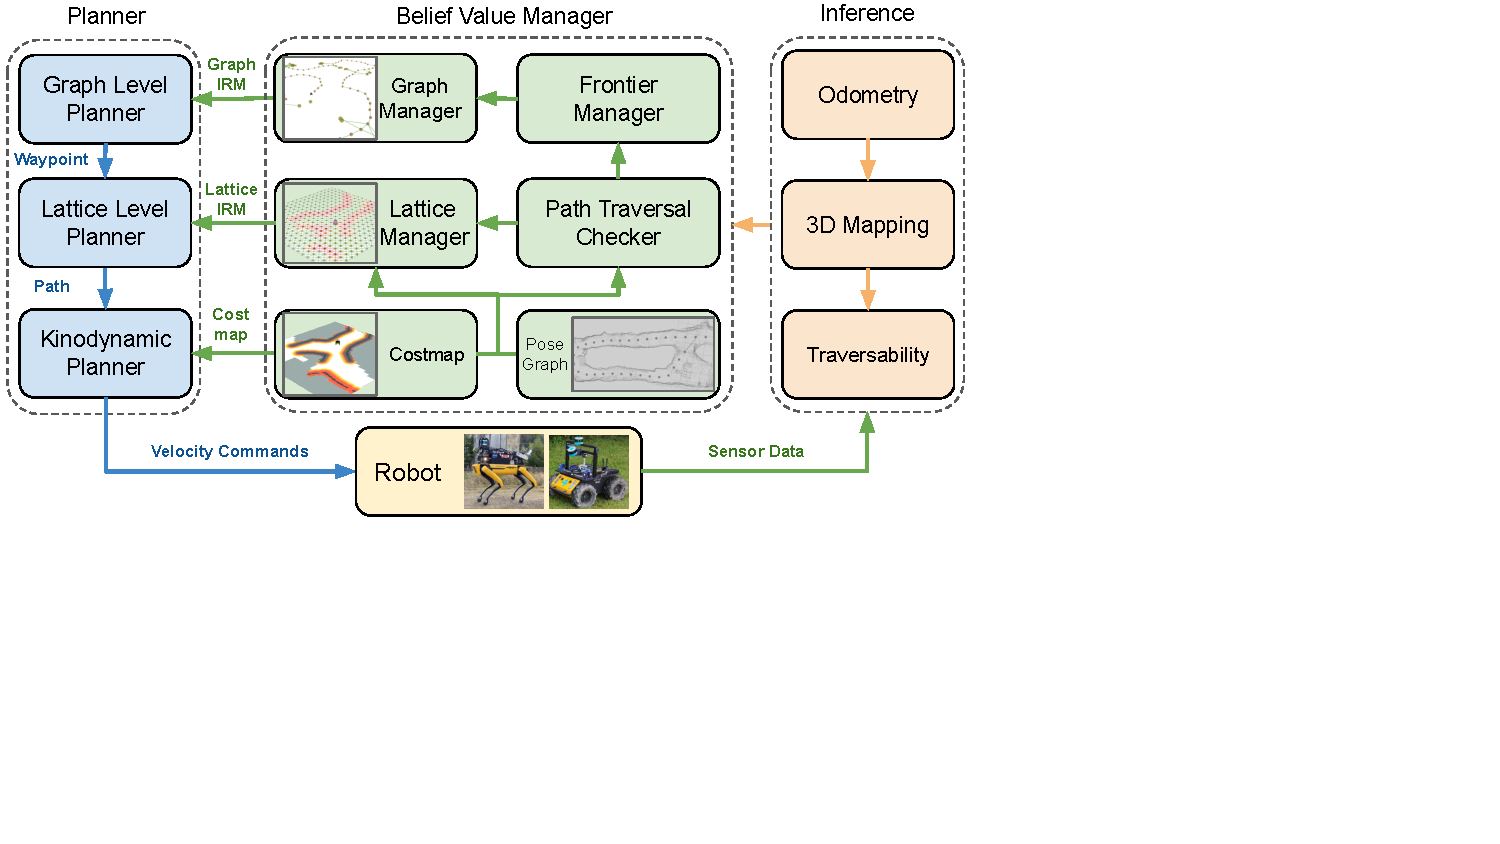
\includegraphics[width=.55\textwidth,trim={0 5.5cm 9.0cm 0},clip]{figures/SystemOverview.pdf}
  }
  \quad
%   \subfloat[Visualization of hierarchical IRMs]{%
%   \subfloat[Hierarchical IRMs]{%
  \subfloat[Graph/Lattice IRMs\label{fig:irms}]{%
    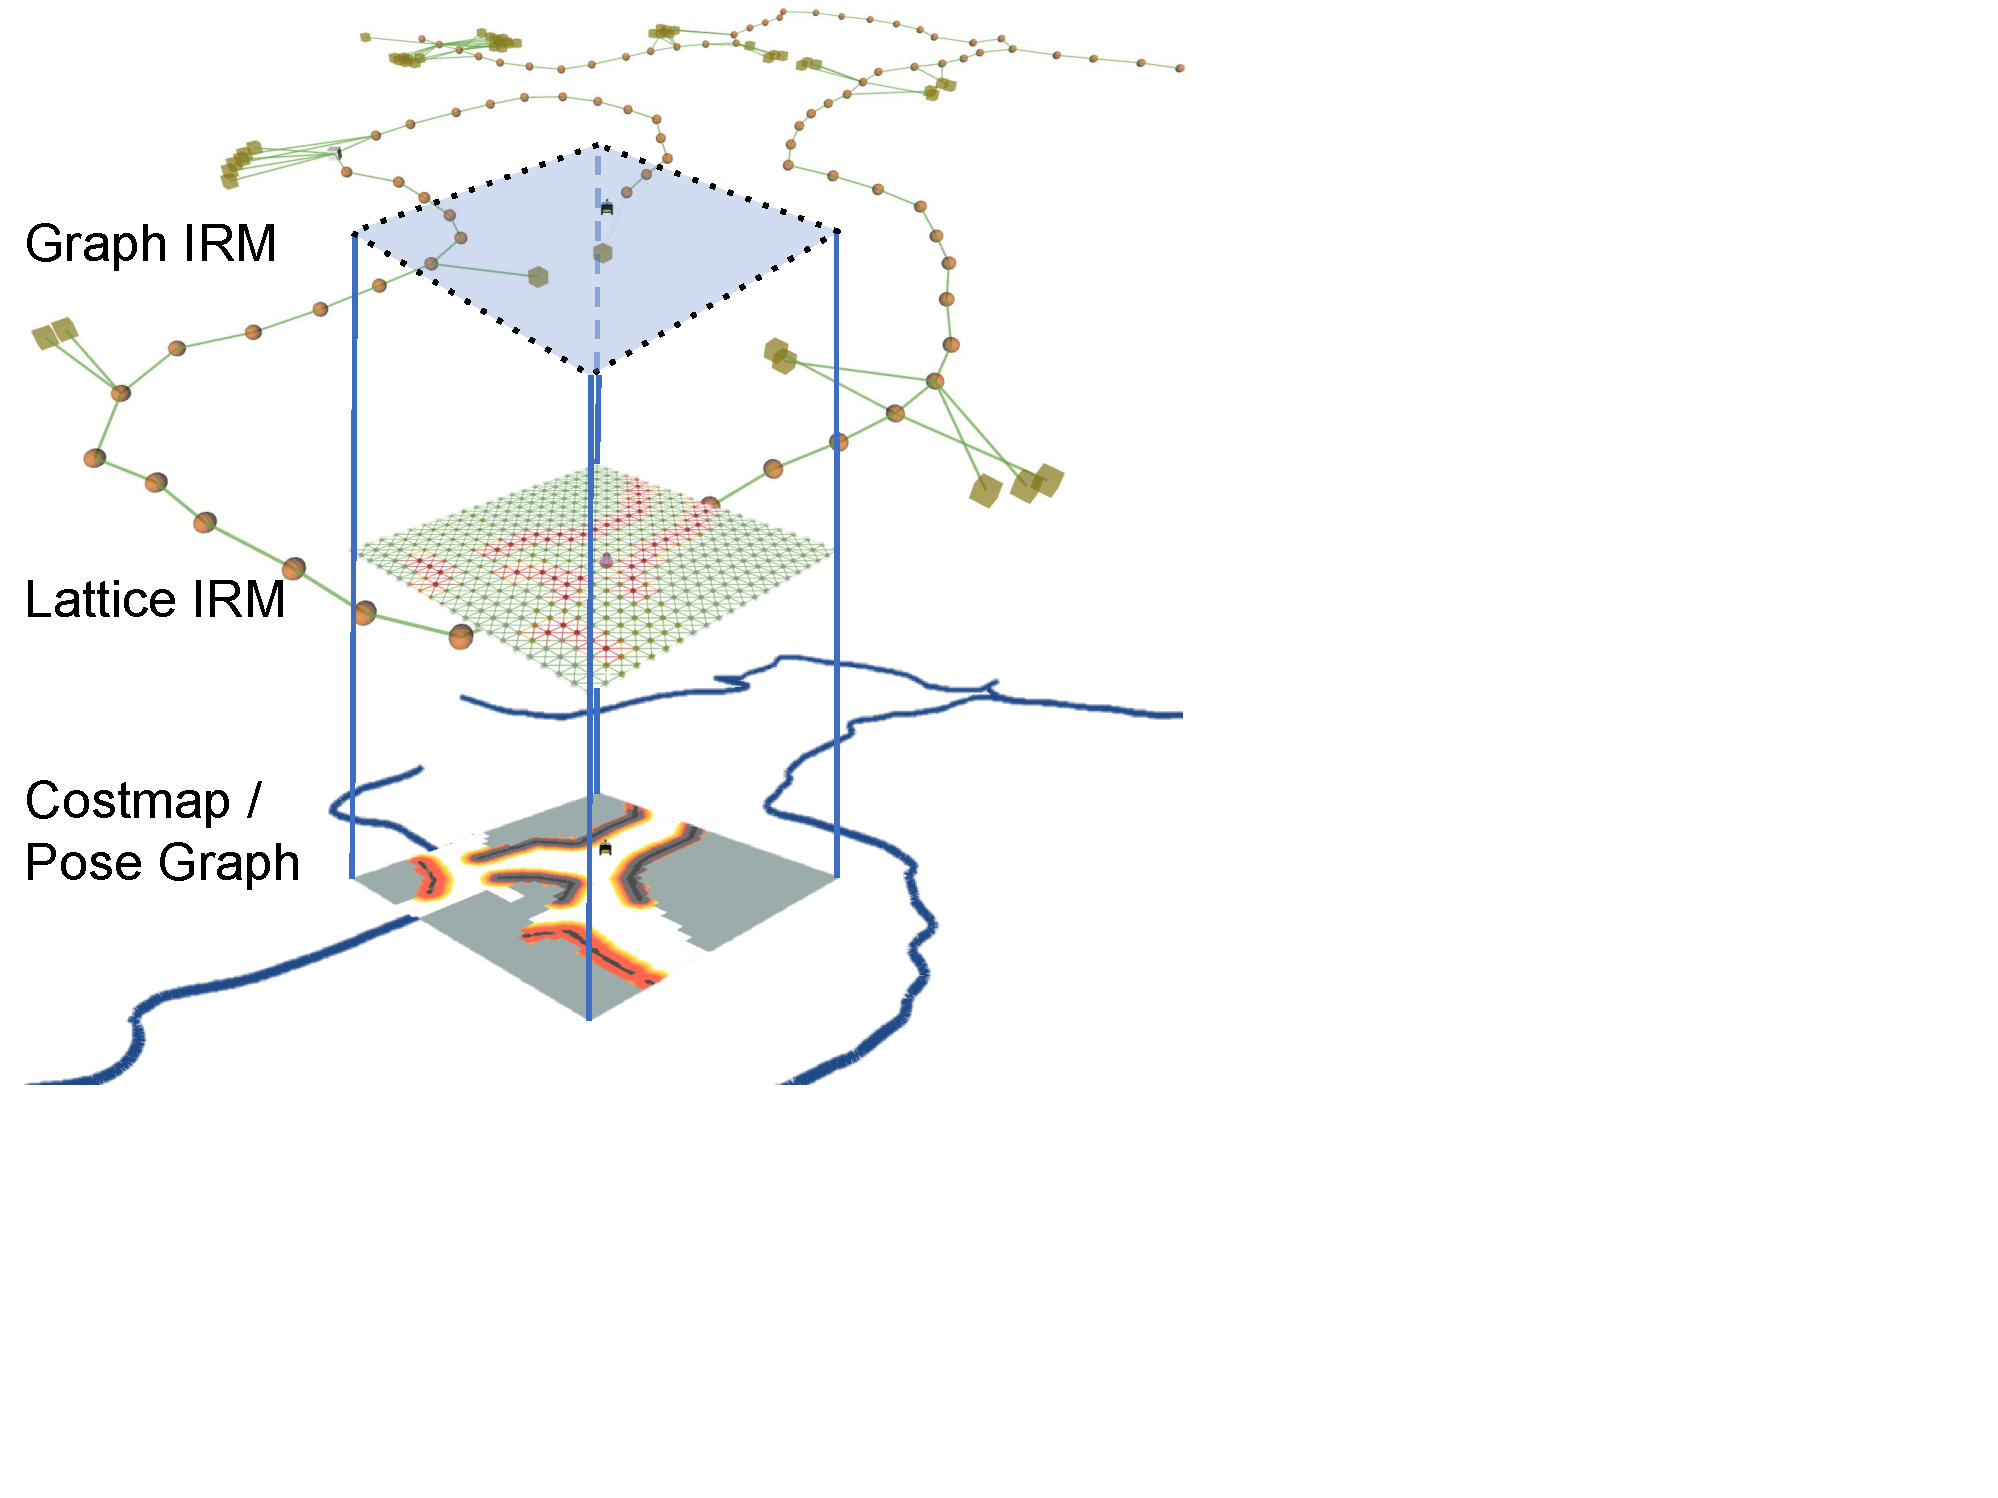
\includegraphics[width=.30\textwidth,trim={0 7cm 16cm 0},clip]{figures/graph-lattice-map.pdf}
  }
  \caption{Overall framework of hierarchical Information RoadMaps (IRMs) and POMDP planners.}
  \label{fig:firstPage}
\end{figure}


% \begin{figure}[t!]
%   \centering
%   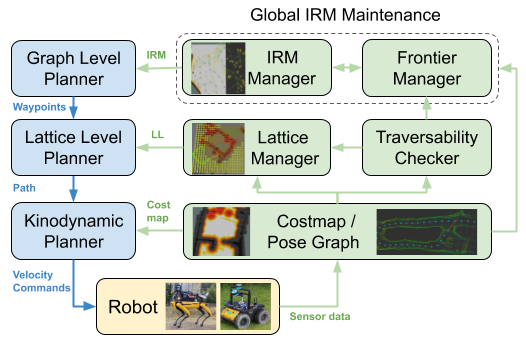
\includegraphics[width=.6\textwidth,trim={0 0 0 1.0cm},clip]{figures/SystemOverview.png}
%   \caption{System diagram of the overall PLGRIM framework.}
%   \label{fig:system_overview}
% \end{figure}

% \begin{figure}[t!]
%   \centering
%   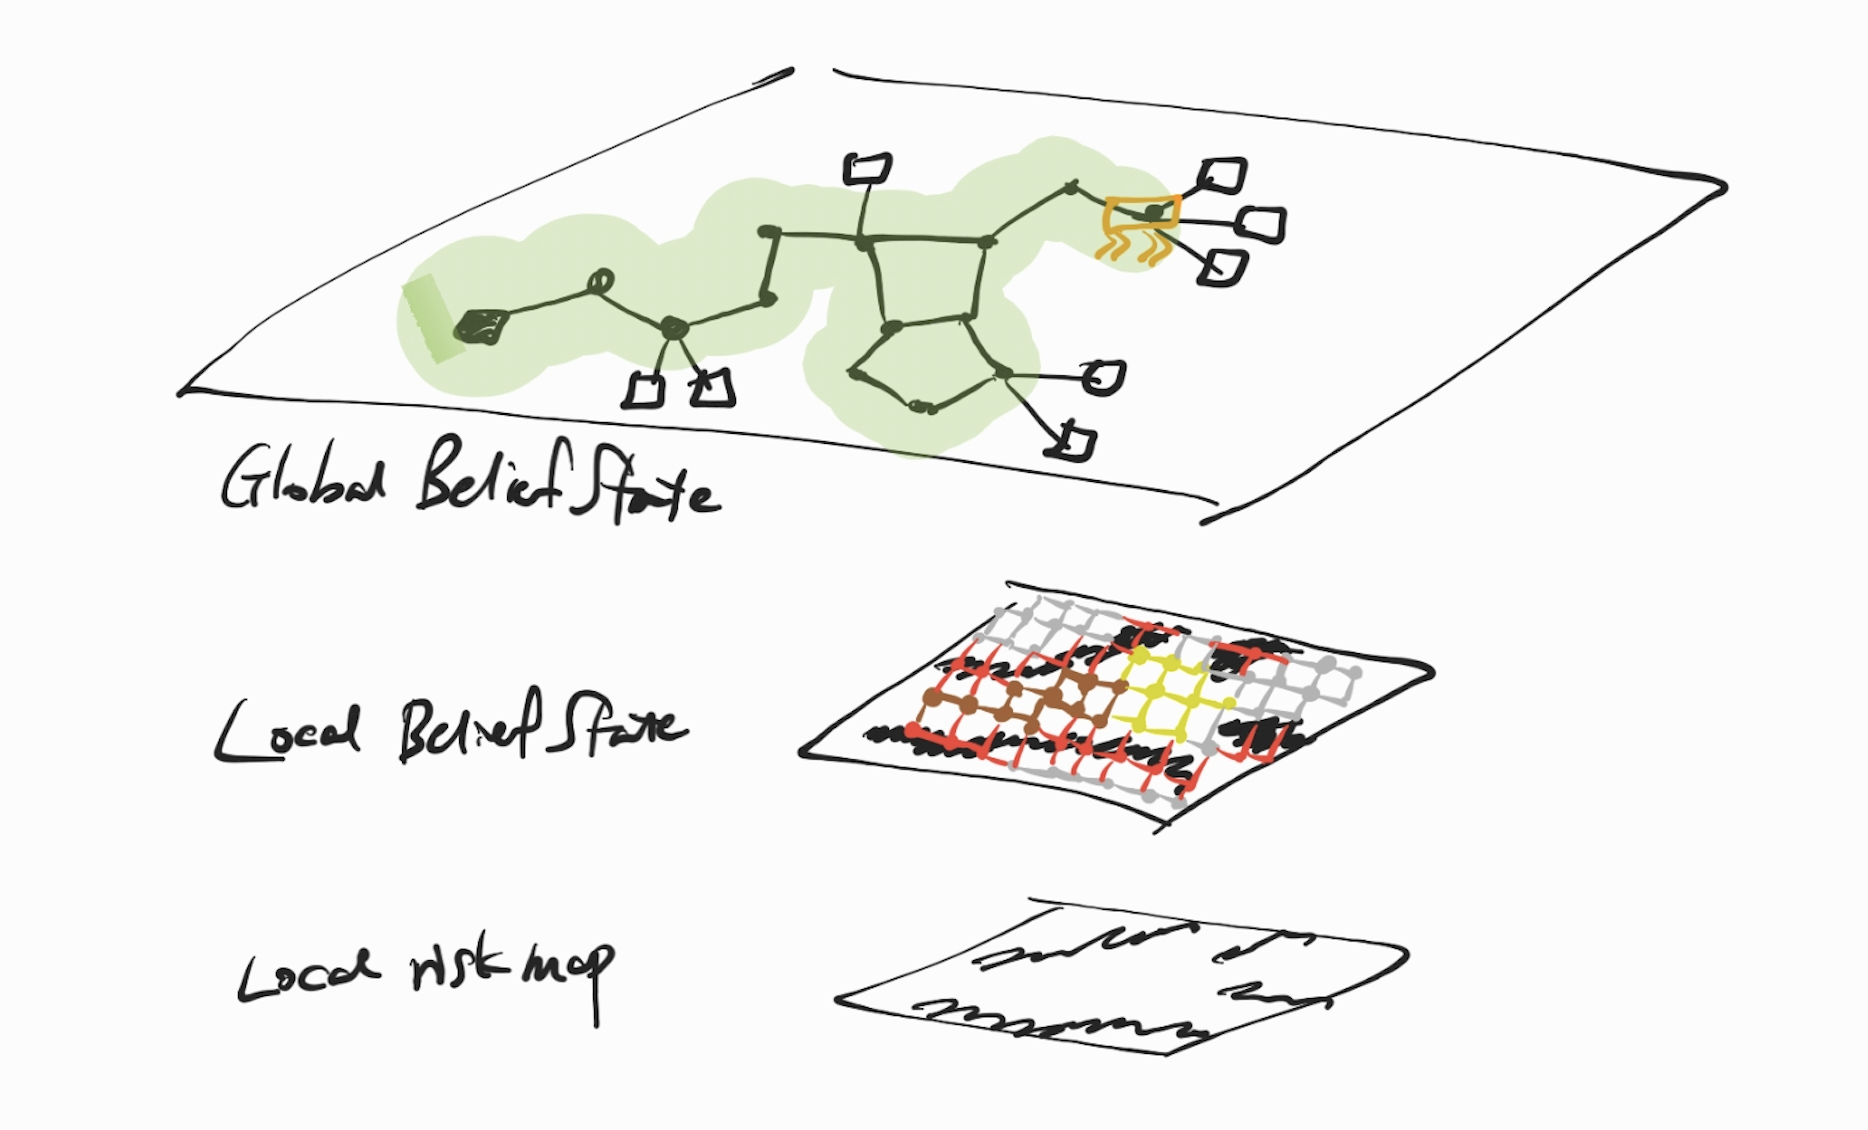
\includegraphics[width=.6\textwidth]{figures/sketch_hierarchical_belief_space.png}
%   \caption{Illustration. [TODO] Visualize the planned path in each level.}
%   \label{fig:illustration}
% \end{figure}

%\ph{Gap in the state-of-the-art}
Belief value learning in POMDP setting suffers from the curse of dimensionality \cite{KLC98} and curse of history \cite{Pineau03}. Many powerful methods are extending the spatial and temporal horizons of POMDPs with varying degrees of efficiency and accuracy (e.g., \cite{silver2010monte,somani2013despot,bonet1998learning,kim2019pomhdp}). In this paper, we deal with exploration problems with very long time horizons (> 1 hour), large spatial extents (> 10 km$^2$), and high dimensional belief states (including beliefs on the state of the environment), that exacerbates the curses of history and dimensionality when planning robot behaviors over the belief space.
%

%\ph{Contributions}
To address this problem, we introduce several key spatial and temporal approximations of the robot policy space to enable computational tractability while constructing an online and real-time solver.
%search space.  This decomposition allows us to approximately solve the optimization problem in a computationally tractable manner.  
Spatially, we decompose the belief space into task-relevant partitions of the space,
%into a robot and task-relevant graph structure 
enriched with environment map estimates. %, which reduces our search space for good policies, 
The partitioning structure is called an Information Roadmap (IRM) (Fig.~\ref{fig:irms}). Temporally, we decompose the problem into a long-range (global) IRM which spans the entirety of the known environment, and a robot-centered short-range (local) IRM. % with fixed size. 
We then propose a receding-horizon-control (RHC)-based solver to address the planning over this hierarchical POMDP structure % problem in a receding horizon fashion, 
in real time.

%\ph{Outline}
Section~\ref{sec:related_work} presents the related work and Section~\ref{sec:ECSPasPOMDP} formalizes the problem.
We propose the hierarchical belief learning and coverage planning framework in Section~\ref{sec:plgrim}. Experimental results in simulation and on physical robots are presented in Section~\ref{sec:exp_results}.% validating our method, and Section~\ref{sec:conclusion} concludes this paper.


%%%%%%%%%%%%%%%%%%%%%%%%%%%%%%%%%%%%%%%%%%%%%%%%%%%%%%%%%%%%%%%%%%%%%%%%%%%%%%%%
\section{Related Work}\label{sec:related_work}
%\ph{Coverage--Frontier-based exploration}
Frontier-based exploration is a widely used approach for autonomous exploration (e.g., \cite{yamauchi1997frontier,tao2007motion,keidar2012robot,heng2015efficient,gonzalez2002navigation,grabowski2003autonomous}). By continuing exploration until exhausting all remaining frontiers, frontier-based approaches can guarantee \textit{completeness} of the coverage of reachable spaces.  These methods typically rely on myopic (e.g., one-step) look-ahead greedy policies, selecting the best frontier upfront. Hence they can be subject to local minima and provide suboptimal solutions in time.

%\ph{Coverage--(Model-free) RL-based approaches}
Model-free reinforcement learning (RL) has been applied to coverage and exploration problems (e.g., \cite{pathak_icm, rnd,burda2018study,ECR2018}). In this setting, the typical approach is to find a policy which maps sensor data to actions, to maximize the reward. When it comes to long-range and large-scale, and (possibly safety-critical) missions on physical robots, collecting necessary data for this class of methods can be a significant challenge.

%\ph{Coverage--(Model-based RL) POMDP approaches}
POMDP-based approaches generate a non-myopic policy by considering long-horizon action sequences (e.g., \cite{kurniawati2011motion}, \cite{bai2015intention}), interactively learning the value function, and returning the best action sequence that maximizes the accumulated rewards. Different methods have reduced the complexity of the POMDP problem in coverage and exploration problems. \citet{indelman2015planning} and \citet{martinez2009bayesian} employed a direct policy search scheme with a Gaussian belief assumption. \citet{Lauri2016planning} extended this to non-Gaussian beliefs using the POMCP (Partially Observable Monte-Carlo Planning) solver. % algorithm that uses a Monte-Carlo Tree Search \cite{silver2010monte}.
%In this work, we aim at scaling the solution even further to enable solutions for hte missions fo interste that are longer and larger than mission 
However, when it comes to aforementioned missions of interest, the current approaches do not scale well due to the curse of history and dimensionality \cite{Pineau03}.

%\ph{Large scale--Hierarchical approaches}
Hierarchical planning structures \cite{kaelbling2011planning} aim to tackle larger problems by employing multiple solvers running at different resolutions.  
%
In the coverage and exploration context, \citet{umari2017autonomous} applies hierarchical planning to frontier-based exploration, while  \cite{dang2019explore} extends the lower level module to a more sophisticated frontier selection algorithm considering the information gain along each path. \citet{Lauri2016planning} replace the lower level module with a POMDP-based planner, to improve local coverage performance with non-myopic planning. \citet{kim2019bi} propose a hierarchical online-offline solver for risk-aware navigation. \citet{vien2015hierarchical} propose a hierarchical POMCP framework which outperformed Bayesian model-based hierarchical RL approaches in some benchmarks.

\section{Exploratory Covering Salesman Problem}
\label{sec:ECSPasPOMDP}
In this section, we introduce the coverage problem as a variant of the traveling salesman problem, and show how we formalize it as a POMDP. We then discuss the challenges and our approach. %how the exact solution to this problem can easily become intractable.  

\ph{Covering Salesman Problem (CSP)} Given a known environment represented by an abstract graph structure $W = (V, E)$, with free and occupied nodes $V_{free}\cup V_{occ} = V$, the traditional coverage problem aims to find a sequence of nodes and edge traversals that pass through all free nodes $V_{free} \subseteq V$.  By incorporating a sensor field-of-view $F:V\rightarrow \mathcal{P}(V)$, which maps each node to a subset of "visible" nodes, and adding the objective of minimizing travel distance, the coverage problem can be seen as a generalization of the traveling salesman problem -- the \emph{covering salesman problem} (CSP).  In the CSP, the objective is to determine the minimum length path through a subset of nodes $\{v_i\}_i \subseteq V_{free}$ such that every free node is within the accumulated sensor field-of-view: $V_{free} \subseteq \cup_i F(v_i)$.
In this paper, we further modify the CSP by assuming that the environment $W$ is not known a priori, which we call an \emph{exploratory covering salesman problem} (ECSP).  After incorporating a consideration of motion and sensing uncertainty of the agent, we can cast the ECSP as a POMDP problem with a reward function designed for coverage, which we will refer to as \emph{ECSP-POMDP} hereafter.

\ph{ECSP-POMDP Elements} A POMDP is described as a tuple $\langle \mathbb{S}, \mathbb{A}, \mathbb{Z}, T, O, R \rangle$, where $\mathbb{S}$ is the set of states of the agent and world, $\mathbb{A}$ and $\mathbb{Z}$ are the set of robot actions and observations. At every time step, the agent performs an action $a \in \mathbb{A}$ in state $s$ and receives an observation $z \in \mathbb{Z}$ resulting from the agent's perceptual interaction with the environment. The motion model $T(s, a, s') = P(s'\,|\,s, a)$ defines the probability of being at state $s'$ after taking an action $a$ in state $s$. The observation model $O(s, a, z) = P(z\,|\,s, a)$ is the probability of receiving observation $z$ after taking action $a$ in state $s$. The reward function $R(s,a)$ returns the expected utility for executing action $a$ in state $s$.

\ph{State} We define the system (robot-world) state as a 2-tuple $s = (W, Q) \in \mathbb{W}\times\mathbb{Q} =  \mathbb{S}$ consisting of the robot state $Q$ and the regions of the world have been observed (covered) by the robot $W$. The world representation can be further decomposed as $W = (W_{occ}, W_{cov})$ where $W_{occ}$ describes a representation of the geometry of the world, and $W_{cov}$ encodes which regions of the world have been observed by the robot.  For example, $W_{occ}:\mathbb{Q}\rightarrow\{0,1\}$ can be a mapping from pose to the set $\{0,1\}$, where $W_{occ}(Q) = 0$ if the location is free and $W_{occ}(Q) = 1$ if the location is occupied (and similarly for $W_{cov}$).  We also denote the ground truth occupancy of the world as $W_{occ}^{GT}$.
% The underlying ground truth (complete) world is denoted by $W_{occ}$. For example, $W_{occ}:\mathbb{Q}\rightarrow\{0,1\}$ can be a binary mapping, where $W_{occ}(Q) = 0$ if the location is free and $W_{occ}(Q) = 1$ if the location is occupied (and similarly for $W_{cov}$).  %We also denote the ground truth occupancy of the world as $W_{occ}^{GT}$.

\ph{Belief State} Since the state of the world is not fully observable, the agent maintains a belief state $b_t\in \mathbb{B}$ defined as the posterior distribution over all possible states conditioned on past actions and observations at time $t$. The belief over state $s$ is $b_{t} = P(s \,|\, a_{0:t-1}, z_{1:t})$. The ESCP belief state is a 2-tuple $b_t = p(s_t) = p(W,Q)$.

\ph{Transition Model} Given an action $a$, the estimated transition model $T$ maps the robot and world state $s = (W, Q)$ to the subsequent state $s' = (W', Q')$, i.e., $T(s, a, s'; \, W_{occ}^{GT})$. 
The transition model is parametrized by ground truth world map $W_{occ}^{GT}$, which represents the generative model (in simulation or physical robot motion). %It encodes the traversability risk of an action $a \in \mathbb{A}$. 
The model $W_{occ}^{GT}$ encodes the true traversability information and determines if the robot can or cannot transition along the edge $e$ induced by action $a$.% and, consequently, the state does not change: $s = s'$.

\ph{Observation} Upon taking an action $a$ in state $s$, the robot receives an observation of the robot state $Q$ and a partial observation of the world state $W$. Given a robot state $Q$, the robot observes areas of the world within the field-of-view of its sensors.  The observation model is denoted by $  O(z | s, a; \, W_{occ}^{GT})$
where $O$ provides information about $W_{cov}$.% within the field-of view, which depends on a ray-casting model.

\ph{Traditional Map Representation} Grid maps are a common representation of the world state $W$ in robotics. %(which we introduced as having a continuous domain, i.e. $W:\mathbb{Q}\rightarrow \{0,1\}$)
By using grid cells $\bar{W}=\{m_i\}_i$ where $m_i$ represents the world state (occupancy, coverage, etc.) at the $i$-th cell, the world state is reduced to a discrete domain.  In this work, we lightly assume the presence of a mapping and costmap-generating module which creates a local map $\bar{W}$.  
In order to compute the posterior probability $p(\bar{W} | z_{1:t}, Q_{1:t})$ of the whole map $\bar{W}$, given the robot's measurements $z_{1:t}$ and trajectory $Q_{1:t}$, the binary cell states are traditionally approximated by assuming full independence between them \cite{TBF05,elfes1990stochastic}. Note that in this work, the resolution of $\bar{W}$ is about of 10cm for a 1m-sized robot.

\ph{Pose Graph} In addition to the grid map representation of the environment, we employ a \textit{pose graph} \cite{thrun2002probabilistic}, where $\mathcal{PG} = p(Q_{0:t})$ is the belief over the path history taken so far.  This pose graph is generated by a SLAM algorithm and should run in realtime to support our planning architecture.  %In practice we may simplify our representation of $\mathcal{PG}$ by approximating it with the maximum likelihood estimate.

\ph{Reward} The one-step reward is computed as a function of the information gain and cost associated with an action:
\begin{align}
    {R}(s, a) = \mathcal{F}\Big[\, \textit{InfoGain}(W_{cov}, z), \; \textit{Cost}(W_{occ}, a) \, \Big]%: \, \mathbb{S} \times \mathbb{A} \rightarrow \mathbb{R} 
\end{align}
Information gain is defined as the marginal gain of information: $\textit{InfoGain}(W_{cov}, z) = I(W_{cov} \cup z) - I(W_{cov})$, since the benefit of being in a state $s$ is dependent on whether the robot has already observed neighboring areas in the world. \ali{The cost of an action $Cost$ is a function of the world geometry $W_{occ}$ since this sub-state informs both the required actuator output (path length and velocity) and the proximity to the actuator's limitations (traversability risk) required to execute an action.}

\ph{ESCP-POMDP} We define a belief policy as a function $\pi : \mathbb{B} \rightarrow \mathbb{A}$ which maps each belief state $b$ to an action $a$.  Let the belief reward $r(b,a)=\int_s R(s,a)b(s)ds$ be the expected reward of taking action $a$ at belief $b$.  The optimal policy maximizes the expected discounted sum of future rewards.
\begin{align}
  \pi^*(b) &= \arg\max_\pi \, \mathbb{E} \sum_{t=0}^{L} \gamma^t r(b_t, \pi(b_t)) 
  \label{eq:optimal_policy}
\end{align}
where $\gamma \in (0,1)$ is a discount factor which ensures that immediate rewards have a greater effect on decisions than future rewards. The overall objective is to solve this optimization problem in a computationally tractable way.

\ph{Intractability} 
%Given the high-dimensional grid representation of the world state, 
Eq. (\ref{eq:optimal_policy}) is a highly intractable optimization for large environments. This is because of 1) the high dimension of the belief state $b$, particularly with respect to the belief over the high-dimensional grid representation of the world state $\bar{W}$, and 2) the large timescale $L$ as the complexity of the search space grows exponentially with time. In the next section, we discuss our approach to further decompose and address this problem.


%%%%%%%%%%%%%%%%%%%%%%%%%%%%%%%%%%%%%%%%%%%%%%%%%%%%%%%%%%%%%%%%%%%%%%%%%%%%%%%%
\section{PLGRIM: Hierarchical Coverage Planning on Information Roadmaps}
\label{sec:plgrim}

%\ph{Our Contributions} 
To obtain a tractable solution to the ESCP problem in Eq. (\ref{eq:optimal_policy}), we propose a novel approach in which we 1) introduce a hierarchical approximation of the belief space $b=p(W,Q)$ to reduce the policy search space, and 2) introduce a hierarchical RHC-POMCP solver to quickly find non-myopic solutions on local to global scales in real-time.

\ph{Architecture}  We decompose the problem into tractable subproblems by introducing spatial and temporal abstraction which enable efficient and reactive robot behaviors on very large scales (kms).  The hierarchical planner has two cascaded layers with different environment representation scales. The higher layer, which we call a \emph{graph-level planner}, employs a sparse graph structure of dynamic size which captures the connectivity of the free space in the known part of the environment. The lower layer, which we call a \emph{lattice-level planner}, employs an agent-centered dense grid structure of fixed dimensions that moves with the robot (see Fig.~\ref{fig:system_overview}). %6

\subsection{Hierarchical Belief Space Representation} 

\ph{Belief Encoding} Both the graph-level planner and lattice-level planner use a graph-based abstraction of the world state $W$.  We call these graph-based approximations an \textit{Information Roadmap (IRM)}. %\cite{agha2014firm}.
We use super-scripts $(\cdot)^g$ or $(\cdot)^l$ as needed to describe objects specific to the graph-level or lattice-level respectively. We describe the graph-level IRM first, but most discussions apply to the lattice-level IRM too. Let $V^g=\{v_i\}_i$ denote a set of robot poses $v_i\in \mathbb{Q}$.  Then for each pose $v_i\in V^g$ we construct an approximation of $W(v_i) \approx W^g(v_i)$, with $W_{occ}^g(v_i) = \{0,1\}$ and $W_{cov}^g(v_i) = \{0,1\}$.  %This approximation can be constructed by finding the maximum value $W_{occ}(v_j)$ for all $v_j$ in a neighborhood of $v_i$, or some other approximate method.  We also can approximate $W_{cov}^g$ as a function of the poses $V^g$ and the pose graph $\mathcal{PG}$. 
For details on computing these approximations for both graph-level and lattice-level, see the supplemental material.  We then construct an approximate graph-level belief $b^g=p(W^g, Q)$.  By assuming independence between variables, this belief can be decomposed as $b^g=p(Q)\prod_i p(W_{occ}^g(v_i))$.  Additionally, to create a meaningful decomposition of the action space, we construct edges $E^g=\{e_{ij}\}_{i,j}$ which connect the nodes $v_i, v_j$.  In doing so, we create a graph structure $G^g=(V^g, E^g)$ representation of the world.  We associate to the edges transition probabilities as well as other quantities of interest (e.g. risk, cost of traverse, etc).

Fig. \ref{fig:system_overview} illustrates the process by which the 3D volumetric information $W$, acquired from raw sensor data, is approximated into discrete probability distributions over occupancy and coverage. 
Therefore, we have approximated and discretized the belief space $b^g\in\mathbb{B}^g\subset\mathbb{B}$ and $b^l\in\mathbb{B}^l\subset\mathbb{B}$ for the graph and lattice-level planners to act on.

%\ph{POMDP Specifics}
For each planning problem in the hierarchy we define a sub-POMDP problem over the graph representation.  The details of these problems differ in terms of the definitions for transition models $T^g(\cdot),T^l(\cdot)$, observations $O^g(\cdot),O^l(\cdot)$, and rewards $R^g(\cdot),R^l(\cdot)$.  We detail the particular design choices used in this work in the supplementary material, and give the general framework here.

\subsection{Hierarchical Policy Formulation}
\label{sec:hierarchical_policy}
\ph{Policy} We define a graph-level policy as a mapping from the graph-level belief state $b^g$ to a goal-related parameter $\theta^g \in \Theta^g$ 
\begin{align}
    \pi^g : \mathbb{B}^g \to \mathbb{A}^g, \; \mathbb{A}^g = \Theta^g\ .
\end{align}
The action space $\Theta^g$ encodes a global, non-myopic task, and serves as an input to the lattice-level policy: 
\begin{align}
    \pi^l: \mathbb{B}^l \times \Theta^g \to \mathbb{A}^l\ .
\end{align}
The output of the lattice-level policy is a controller to move the robot (e.g. a waypoint or path for a controller to track, or parameters for a feedback policy that generates control commands).

We define an overall policy $\pi \in \Pi$ generated by combining the graph-level policy $\pi^g$ and the lattice-level policy $\pi^l$:
\begin{align}
    \pi(b) = \pi^l(b^l; \, \pi^g(b^g)) = \pi^l(b^l; \, \theta^g) : \, \mathbb{B}\rightarrow \mathbb{A} 
\end{align}

\ph{Reward} The one-step reward received by the agent upon taking a lattice-level policy $a^l$ in belief $b^l$ is:
\begin{align}
    r^l(b^l, a^l) = r^l(b^l, \pi^l(b^l; \theta^g) = r^l(b^l, \pi^l(b^l; \pi^g(b^g)))
\end{align}

\ph{Policy} We define the hierarchical policy of the graph and lattice level policies as:
\begin{align}
  \pi^{*}(b) &= \arg\max_\pi \, \mathbb{E} \left[ \sum_{t=0}^{L} \gamma^t r^l(b^l_t, \pi^l(b^l_t; \pi^g(b^g_t)) \right]
  \label{eq:optimal_policy_unified}
\end{align}

\ph{Policy decomposition and interaction} In this work, we choose to represent the graph planner's output actions $\theta^g$ as nodes $v^g_i \in V^g$ in the graph-level IRM $G^g$. These nodes are passed to the lattice planner, whose objective is to explore locally. Similarly, the lattice-level planner's output actions are nodes $v^l_i \in V^l$ in the lattice-level IRM $G^l$.  In order to maintain a tractable problem in both the graph and lattice levels, we decouple the policies in the following manner:  The lattice-level planner typically sends its action $v^l_i$ to the kinodynamic planner, which produces velocity commands for the robot.  However, if there is no exploration possible in the lattice map, the lattice-level planner passes along the graph-level planner's action $v^g_i$ to the kinodynamic planner, which encodes a new area in the graph-level IRM for the lattice-level planner to explore.  At any time the lattice-level planner may decide to continue exploring on the lattice-level IRM.  In this manner, we encourage high-fidelity local exploration without sacrificing large-scale, globally optimal decision making.

In the next section, we describe the POMDP solver approach to optimizing the global and local policies of Equation \ref{eq:optimal_policy_unified}.


%%%%%%%%%%%%%%%%%%%%%%%%%%%%%%%%%%%%%%%%%%%%%%%%%%%%%%%%%%%%%%%%%%%%%%%%%%%%%%%%
\subsection{Real-time Hierarchical Solver for ECSP-POMDPs}

% \textbf{Separate POMCP algorithm -- SIMULATE ROLLOUT SEARCH}



% Amanda/David Version
%%%%%%%%%%%%%%%%%%%%%%%%%%%%%%%%%%%%%%%%%%%%%%%%%%%%%%%%%%%%%%%%%%%%%%%%%%%%%%

\begin{algorithm}[t!]
\caption{Hierarchical Coverage Planner}
\label{alg:hierarchicalPlanner}
\begin{multicols}{2}
\begin{algorithmic}
\STATE \underbar{\textbf{Function HierarchicalPlan}}
\item \textbf{input: }Beliefs $b^g$, $b^l$ of states $s=(G, Q)$
\item \textbf{input: }World configuration $W$
% \item \textbf{input: }Optional rollout policy $\pi_{rollout}$
\REPEAT
    \STATE \textbf{\# Global level planner}
    \item  Obtain world information map
    \item Estimate $\hat{\mathcal{G}}^g$
    \item $\theta^l_{t:T} \gets \textsc{POMCP}(b^g, \hat{\mathcal{G}^g}, \pi_{rollout})$
    \STATE \textbf{\# Low level planner}
    \item Obtain local information map
    \item Estimate $\hat{\mathcal{G}}^l$
    \item $a_{t:T}^{*l} \gets \textsc{POMCP}(b^l;\hat{\mathcal{G}}^l, \theta^l_{t:T}, \pi_{rollout})$ 
    % \item \#learn value function and get best actions
    \STATE \textbf{\# Executive}
    \item Execute $a_{t:T}^{*l}$
    \item Obtain $z$ from sensors
    \item Update $Q$, $W$
\UNTIL timeout
\end{algorithmic}

\begin{algorithmic}
\STATE \underbar{\textbf{Function POMCP}}
\STATE \textbf{input: }Initial belief state $b_0$
\STATE \textbf{input: }Estimated generative model $\hat{\mathcal{G}}$
\STATE \textbf{input: }Optional rollout policy $\pi_{rollout}$
% \STATE
\STATE Initialize empty MCTS tree $T_r$
\REPEAT
    % \item Initial state $s_0 \sim b_0$
    \item \# Run SIMULATE with $\pi_{rollout}$ and $\hat{\mathcal{G}}$ to update $T_r$ with learned value function
    \item $T_r \gets \textsc{SIMULATE}(b_0; \hat{\mathcal{G}}, \pi_{rollout})$
    % \STATE Update the values and the number of visits by backpropagation from the leaf node to the root node
\UNTIL{timeout}
% \item 
\item Extract next N actions $a^*_{1:N}$ from $T_r$ \#N=1 for GLP. For LLP, keep going till leaf node
% \STATE
\RETURN $a*_{1:N}$
\STATE
\STATE
\STATE














% Gautam's Version
%%%%%%%%%%%%%%%%%%%%%%%%%%%%%%%%%%%%%%%%%%%%%%%%%%%%%%%%%%%%%%%%%%%%%%%%%%%%%%

% \begin{algorithm}[t!]
% \caption{Hierarchical Coverage Planner}
% \label{alg:hierarchicalPlanner}
% \begin{multicols}{2}
% \begin{algorithmic}
% \STATE \underbar{\textbf{Function HierarchicalPlan}}
% \item \textbf{input: }Beliefs $b^g$, $b^l$ of states $s=(G, Q)$
% \item \textbf{input: }World configuration $W$
% \item \textbf{input: }Optional rollout policy $\pi_{rollout}$
% \REPEAT
%     \STATE \textbf{\# Global level planner}
%     \item  Obtain world information map
%     \item Estimate $\hat{\mathcal{G}}^g$
%     \item $\theta^l_{t:T} \gets \textsc{POMCP}(b^g, \hat{\mathcal{G}^g}, \pi_{rollout})$
%     \STATE \textbf{\# Low level planner}
%     \item Obtain local information map
%     \item Estimate $\hat{\mathcal{G}}^l$
%     \item $a_{t:T}^{*l} \gets \textsc{POMCP}(b^l;\hat{\mathcal{G}}^l, \theta^l_{t:T}, \pi_{rollout})$ 
%     % \item \#learn value function and get best actions
%     \STATE \textbf{\# Executive}
%     \item Execute $a_{t:T}^{*l}$
%     \item Obtain $z$ from sensors
%     \item Update $Q$, $W$
% \UNTIL timeout
% \end{algorithmic}

% \begin{algorithmic}
% \STATE \underbar{\textbf{Function POMCP}}
% \STATE \textbf{input: }Initial belief state $b_0$
% \STATE \textbf{input: }Estimated generative model $\hat{\mathcal{G}}$
% \STATE \textbf{input: }Optional rollout policy $\pi_{rollout}$
% % \STATE
% \STATE Initialize empty MCTS tree $T_r$
% \REPEAT
%     % \item Initial state $s_0 \sim b_0$
%     \item \# Run SIMULATE with $\pi_{rollout}$ and $\hat{\mathcal{G}}$ to update $T_r$ with learned value function
%     \item $T_r \gets \textsc{SIMULATE}(b_0; \hat{\mathcal{G}}, \pi_{rollout})$
%     % \STATE Update the values and the number of visits by backpropagation from the leaf node to the root node
% \UNTIL{timeout}
% % \item 
% \item Extract next N actions $a^*_{1:N}$ from $T_r$ \#N=1 for GLP. For LLP, keep going till leaf node
% % \STATE
% \RETURN $a*_{1:N}$
% \STATE
% \STATE
% \STATE

%%%%%%%%%%%%%%%%%%%%%%%%%%%%%%%%%%%%%%%%%%%%%%%%%%%%%%%%%%%%%%%%%%%%%%%%%%%%%%

% \\  
% \STATE Function SIMULATE(s,h,depth)
% \WHILE{depth < max depth}
%     \IF{$h \in T$}
%         \item add observation node h to $T_r$
%         \item add action node $ha$ to $T_r \forall a$ actions from h
%         \item return $ROLLOUT(s, h, depth)$
%     \ENDIF
%     \item choose action $a$ with maximum combined reward of exploration + UCT reward
%     \item $(s', o, r) \gets \hat{\mathcal{G}}(s,a)$, $h' = hao$ \# new observation node after taking action a and observing o
%     \item $R \gets r + \gamma\times SIMULATE(s', h', depth+1) $
%     \item update visit counts to observation node $h$, action node $ha$, value function $V(ha)$
%     \item return $R$
% \ENDWHILE
% \\
% \STATE Function ROLLOUT(s, h, depth)
% \WHILE{depth < max depth}
%     \item $a \sim \pi_{rollout}(h)$ \# random action, or your customised domain-specific rollout
%     \item $(s', o, r) \gets \hat{\mathcal{G}}(s,a)$, $h' = hao$ \# new observation node after taking action a and observing o
%     \item return $r + \gamma \times ROLLOUT(s', h', depth+1)$
% \\
% \STATE Function $\hat{\mathcal{G}}$(s, a; $W_{occ}$)
%     \item s' $\gets$ T(s, a, $W_{occ}$)
%     \item o $\gets$ O(s.$W_{cov}$, s'.$W_{cov}$, s'.Q, $W_{occ}$)
%     \item r $\gets$ R(...)
%     \RETURN (s', o, r)
% \ENDWHILE
\STATE
\end{algorithmic}

\end{multicols}

% \begin{algorithmic}[1]

% \Procedure{Roy}{$a,b$}       \Comment{This is a test}
%     \State System Initialization
%     \State Read the value 
%     \If{$condition = True$}
%         \State Do this
%         \If{$Condition \geq 1$}
%         \State Do that
%         \ElsIf{$Condition \neq 5$}
%         \State Do another
%         \State Do that as well
%         \Else
%         \State Do otherwise
%         \EndIf
%     \EndIf

%     \While{$something \not= 0$}  \Comment{put some comments here}
%         \State $var1 \leftarrow var2$  \Comment{another comment}
%         \State $var3 \leftarrow var4$
%     \EndWhile  \label{roy's loop}
% \EndProcedure

% \end{algorithmic}
\end{algorithm}


% \begin{algorithm}[t!]
% \caption{Online Planning using POMCPs}
% \label{alg:pomcp}
% \begin{multicols}{2}
% \begin{algorithmic}
% \REQUIRE initial belief state $b_0$
% \REQUIRE estimated generative model $\mathcal{G}$
% \REQUIRE rollout policy $\pi_{rollout}$ (random or domain-specific)
% \STATE Initialize empty MCTS tree $T_r$, globally accessible
% % \STATE Function POMCP($b_0$)
% \REPEAT
%     % \item Initial state $s_0 \sim b_0$
%     \item \# Run SIMULATE with $\pi_{rollout}$ and $\mathcal{G}$ to update $T_r$ with learned value function
%     \item $T_r \gets \textsc{SIMULATE}(b_0; \mathcal{G}, \pi_{rollout})$
%     % \STATE Update the values and the number of visits by backpropagation from the leaf node to the root node
% \UNTIL{timeout}
% \item Extract next N actions $a^*_{1:N}$ from $T_r$ \#N=1 for GLP. For LLP, keep going till leaf node
% \RETURN $a*_{1:N}$
% % \\  
% % \STATE Function SIMULATE(s,h,depth)
% % \WHILE{depth < max depth}
% %     \IF{$h \in T$}
% %         \item add observation node h to $T_r$
% %         \item add action node $ha$ to $T_r \forall a$ actions from h
% %         \item return $ROLLOUT(s, h, depth)$
% %     \ENDIF
% %     \item choose action $a$ with maximum combined reward of exploration + UCT reward
% %     \item $(s', o, r) \gets \hat{\mathcal{G}}(s,a)$, $h' = hao$ \# new observation node after taking action a and observing o
% %     \item $R \gets r + \gamma\times SIMULATE(s', h', depth+1) $
% %     \item update visit counts to observation node $h$, action node $ha$, value function $V(ha)$
% %     \item return $R$
% % \ENDWHILE
% % \\
% % \STATE Function ROLLOUT(s, h, depth)
% % \WHILE{depth < max depth}
% %     \item $a \sim \pi_{rollout}(h)$ \# random action, or your customised domain-specific rollout
% %     \item $(s', o, r) \gets \hat{\mathcal{G}}(s,a)$, $h' = hao$ \# new observation node after taking action a and observing o
% %     \item return $r + \gamma \times ROLLOUT(s', h', depth+1)$
% % \\
% % \STATE Function $\hat{\mathcal{G}}$(s, a; $W_{occ}$)
% %     \item s' $\gets$ T(s, a, $W_{occ}$)
% %     \item o $\gets$ O(s.$W_{cov}$, s'.$W_{cov}$, s'.Q, $W_{occ}$)
% %     \item r $\gets$ R(...)
% %     \RETURN (s', o, r)
% % \ENDWHILE

% \end{algorithmic}
% \end{multicols}
% \end{algorithm}


\begin{figure}[t!]
  \centering
%   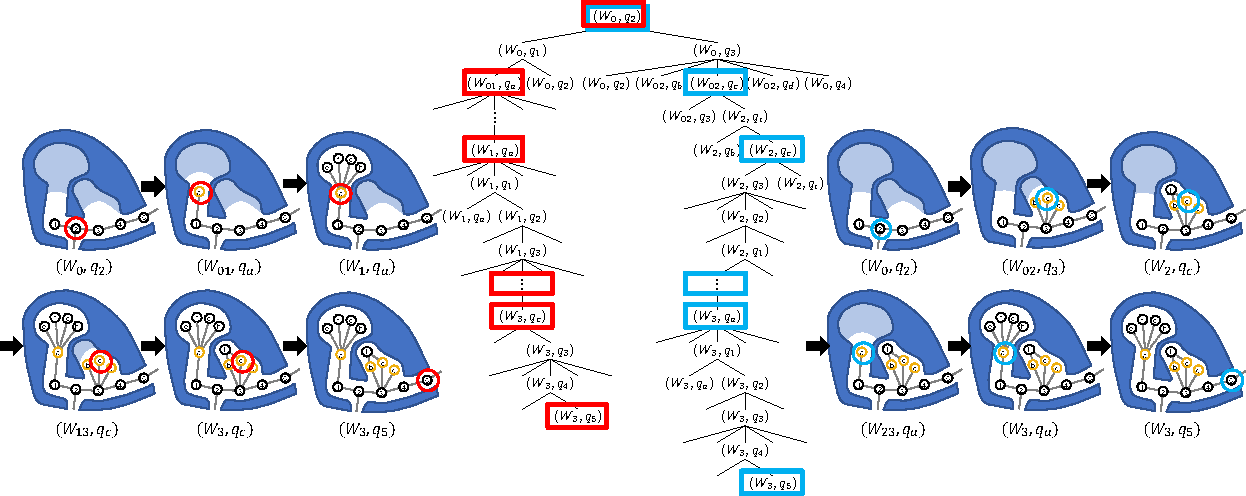
\includegraphics[width=1.0\textwidth]{figures/belief_tree_search.pdf} % without an arrow
  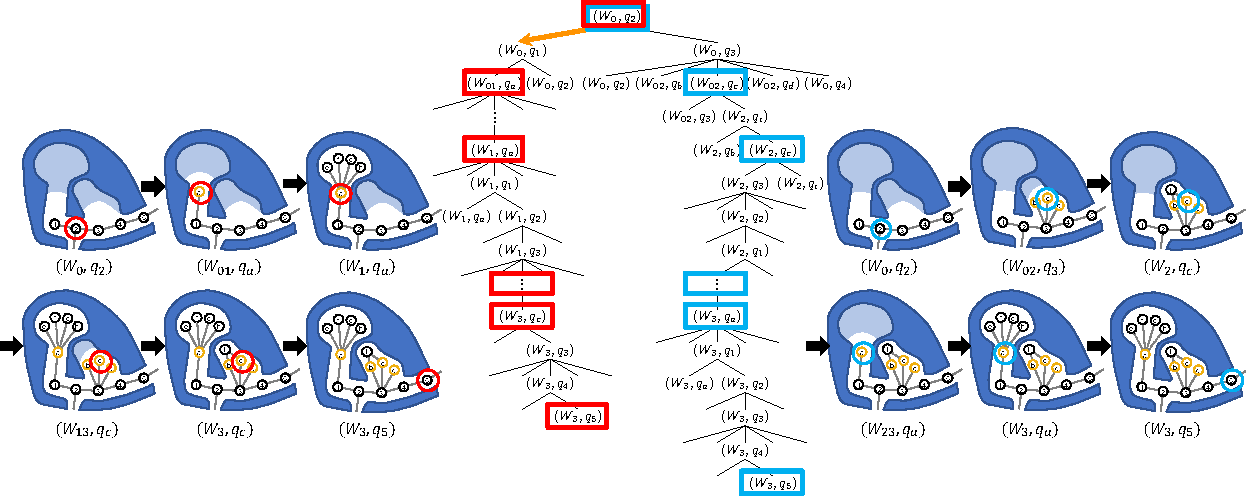
\includegraphics[width=1.0\textwidth]{figures/belief_tree_search_policy.pdf} % with an arrow
  \caption{Illustration of coverage planning with Monte-Carlo Tree Search. A state contains a coverage state of the environment $W$ and a robot pose $q$, and the current state is $(W_o, q_2)$. From forward simulation of possible action sequences and back-propagation of the rewards (e.g., information gain per traversal distance), it can find the best action for the current state, which is \texttt{move-to-$q_1$}.}
  \label{fig:belief-tree-search}
\end{figure}



%\ph{Architecture}
Algorithm~\ref{alg:hierarchicalPlanner} outlines the overall PLGRIM framework for hierarchical coverage planning.  (See also Fig.~\ref{fig:system_overview}.)
At each replanning episode, both the graph-level and lattice-level planners employ a POMDP solver to find a policy at each level, $\pi^g$ and $\pi^l$.  To find these policies we employ POMCP, a Monte-Carlo Tree Search-based POMDP solver \cite{silver2010monte}.  This method requires only a generative model $\mathcal{G}$  (i.e., a black box simulator of the POMDP) instead of explicit mathematical models of the motion and sensing uncertainty. During each simulation, the initial state is sampled from the initial belief state, and the generative model provides a sample of the successor state $s'$, observation $z$, and reward $r$ based on the dynamics of the environment. However, the true state of the world $W^{GT}$ is unknown.  Thus, an approximate generative model $\hat{\mathcal{G}}^g$, $\hat{\mathcal{G}}^l$ is employed for each POMDP (graph and lattice) which uses a posterior distribution of the state  based on sensor data, $p(W^{GT}; a_{0:t-1}, z_{1:t})$ (omitting superscripts $(\cdot)^g, (\cdot)^l$):
\begin{align}
    \hat{\mathcal{G}}(\cdot) = \mathcal{F}(s, a; \, p(W^{GT}; a_{1:t}, z_{1:t})) = \mathcal{F}\big[T(\cdot), O(\cdot), R(\cdot)\big]: \, \mathbb{S} \times \mathbb{A} \rightarrow \mathbb{S} \times \mathbb{Z} \times \mathbb{R}
\end{align}

As the robot moves through the environment, its sensors are used to update the pose-graph $\mathcal{PG}$ and the %kinodynamic 
costmap $\bar{W}$.  These are sent to modules which update the global-level IRM $W^g$ and the lattice-level IRM $W^l$, as well as estimates of the generative models $\hat{\mathcal{G}}^g$ and $\hat{\mathcal{G}}^l$. For details of these modules, see the supplemental material.

\ph{Implementation Details}
The POMCP solver uses Monte-Carlo Tree Search over the belief space of the world. Fig.~\ref{fig:belief-tree-search} shows a sample domain where the robot has covered parts of the world, shown in white. From node 2, the robot runs POMCP with the generative model $\mathcal{G}$, to generate the MCTS tree in the center of the figure. The red path (left) explores node $a$ first and then $c$, before moving onto node 5. The blue path (right) explores node $c$ first and then $a$, before moving onto 5. The solver simulates these sequences and back-propagates the rewards to output the optimal step (\texttt{move-to-$q_1$}) for the robot.

% (See Fig.~\ref{fig:belief-tree-search}). 

\section{Experimental Results}\label{sec:exp_results}

% CONTENTS
% - baseline
%     : may-demo
%     : GLP-MLP
%     : GLP-MLP(custom-rollout)
%         . good custom-rollout suggestions for coverage problem
% - environments
%     : toy example?
%     : mission in sim
%         . open-space (subway station)
%         . cave1
%         . cave2
%     : mission with robot
%         . caltech garden
%         . backyard
% - results
%     : toy example?
%         . average reward for different tree queries (one planning episode)
%         . average reward for different rollout policy (one planning episode)
%     : mission in sim
%         . plots
%         . path
%     : mission with robot
%         . screenshots (robot + irm)
%         . path
%         . plot (planning time, traversal distance, ...)


% SUBWAY
% => Gautam: 10depth-GLP
% => Sung: NBV in subway 2x 2run
% => David: NBV in subway 2x (1000sec~2000sec) 2runs
% => plots
% % : in station 1x size: 3runs for each already

% CAVE
% : cave from the center open space
% => 1-2pm: Kyon MLP/GLP cave.world
% => Amanda: NBV in subway 2x

% ROBOT TEST FIGURE




\subsection{Experimental Setup}

% baseline algorithms (name, approach, ...)

% system config

% experiment environment
% - sim (AWS, ...)
% - robot

% ...

%\ph{Setup}
We validate our proposed framework in a high-fidelity simulation as well as on physical systems. The robot system is a four-wheeled vehicle, equipped with three LiDAR range sensors returning 3D point cloud data. We test in two environments - a maze-like cave of size $400$m$ \times 100$m with complex terrain and topology, including narrow passages, dead-ends, open-spaces, and branches with fluctuating curvature, and a large subway station $120$m $\times 40$m with open spaces as well as narrow passages.  The entire autonomy stack runs in real-time on an Intel Core i7 processor with 32 GB of RAM.

\ph{PLGRIM Specifics}
We set the graph-level planner to use a varying-sized graph of $5$m resolution, and the lattice-level planner to use a 20x20 lattice with $1$m resolution.  The LLP was configured to have a higher planning rate (2Hz) so that the robot's path is quickly updated in a receding horizon fashion to ensure the safety of the vehicle. The LLP's planning horizon was restricted to a predefined number of actions on the lattice as it has fixed dimensions.  In contrast, the length of the GLP's planning horizon was defined as a function of the varying size of the graph. We constructed the graph IRM with two types of nodes: breadcrumbs denoting covered areas of the environment, and frontiers representing the boundary between known and unknown space.  

\ph{Comparison Baseline: Lattice-based Next-Best-View}
Next-best-view (NBV) is a one-step lookahead algorithm that estimates the gain of information associated with moving to a position within the robot's field-of-view $F$. We implemented NBV on the lattice structure by computing the traversal distance (via Dijkstra's algorithm) and information gain associated with each reachable node within $F$. The reward, encoding a trade-off between information gain and traversal cost, was selected as the next position. 

The reward was constructed to encode a trade-off between information gain and traversal cost.

The next position was selected by choosing the node with maximum reward. 

% \ph{Coverage Planner Baseline 2: Graph-based Hierarchical Frontier Selection} 
% Frontiers in the graph encode a gain in spatial information for one lookahead step.  We implemented a hierarchical frontier-based planner where local and global frontiers are myopically selected according to two distinct objective functions. As long as the field-of-view constraints of the local reward function are satisfied, the robot is guided by the local frontier planner. When the constraints are broken, the global frontier planner is initiated and the robot is guided FAR AWAY/GLOBAL. 

\subsection{Simulation Results}

% The autonomous exploration results are presented in this subsection. %shown in Fig.~\ref{fig:may-demo-path} and Fig.~\ref{fig:may-demo-plot}.
We demons
As shown in Fig.~\ref{fig:may-demo-path}, the robot started from the staging area on the left (white open-space area) and autonomously explored the maze-like cave over 800 m in 23 min.
Note that the ground truth environment information is not accessible by the robot.

There are many sharp corned in the environment, where the frontier-based exploration approaches may fail to detect the frontiers and abandon exploring beyond the corner.
However, LLP is able to plan for a longer horizon than frontier-based approaches with high-fidelity traversability information considered, so there was not much issues at sharp corners.
(Note that the orange segment of the path on the right in Fig.~\ref{fig:may-demo-path} did not continue into the corner since the terrain is too rough to traverse.)

There are also many dead-ends in the environment, which may cause the LLP does not see any unexplored area within the local lattice, and thus, the robot gets stuck.
However, thanks to the hierarchical planning framework, GLP successfully guided LLP so that the robot move to unexplored area in the environment, without getting stuck.

\begin{figure}[t!]
  \centering
  \subfloat[Cave world ($250m\times 90m$)]{%
    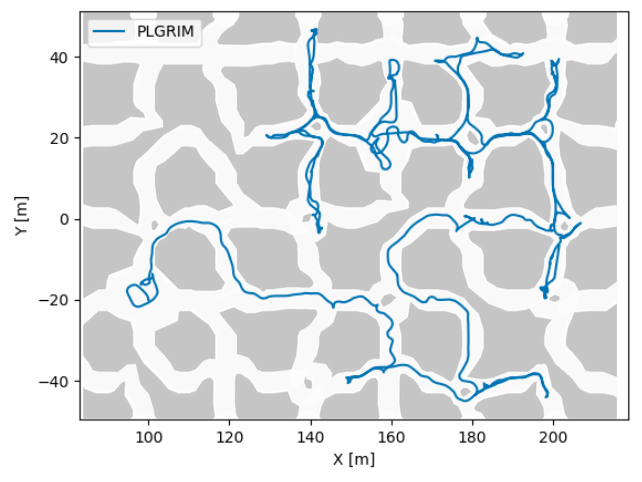
\includegraphics[width=.25\textwidth,trim={2.5cm 2cm 0cm 0cm},clip]{figures/cave_path_c2.png}
    \label{fig:may-demo-path}
  }
  \subfloat[Coverage and distance travelled]{%
    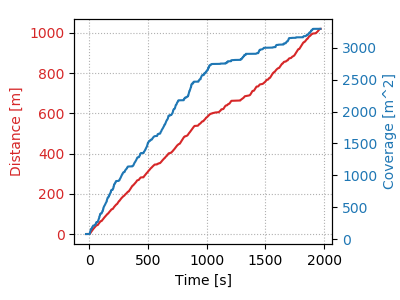
\includegraphics[width=.3\textwidth]{figures/cave_metrics_c2.png}
    \label{fig:may-demo-path-coverage}
  }
  \subfloat[Hardware Testing]{%
    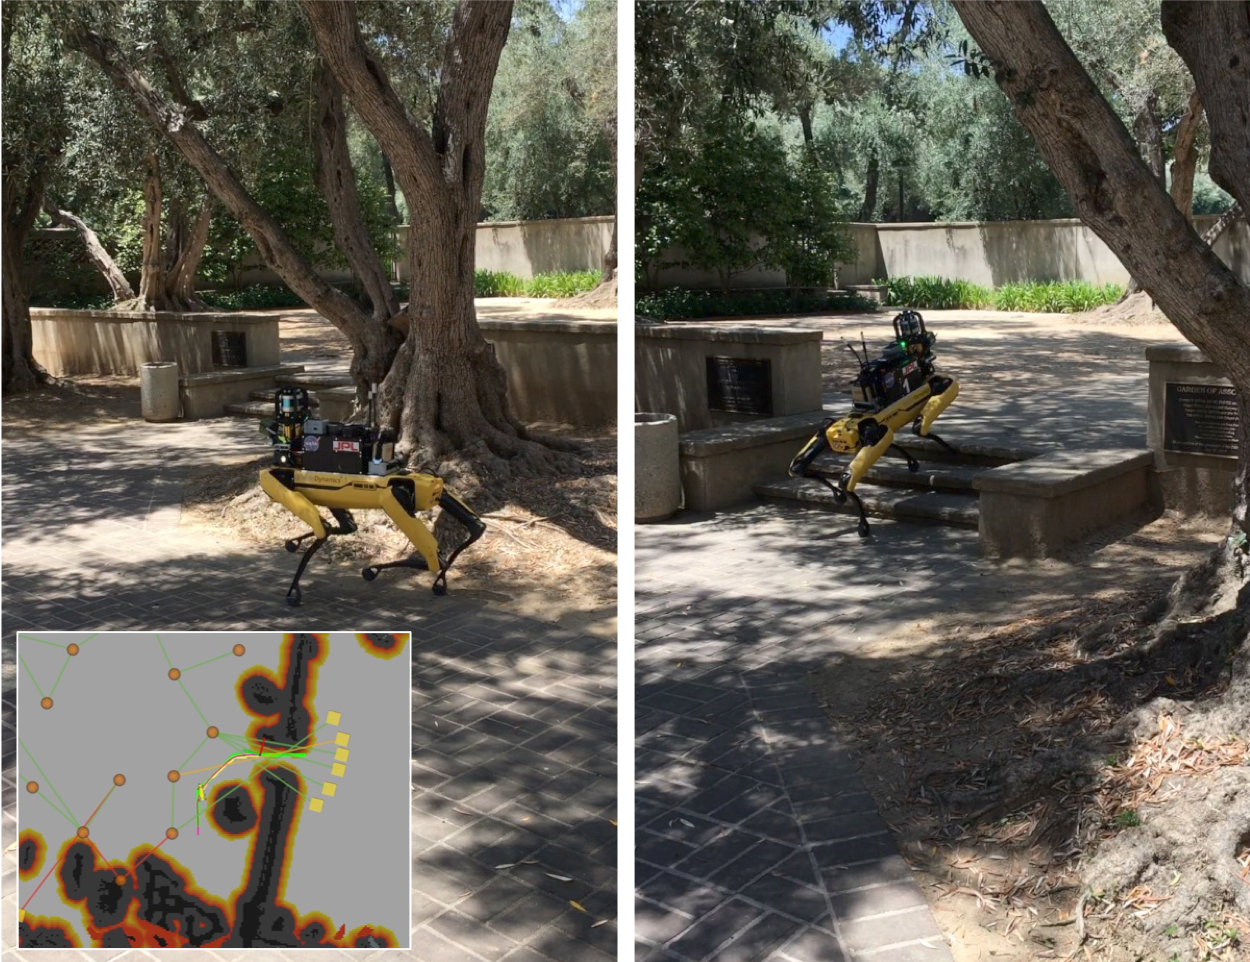
\includegraphics[width=.3\textwidth,trim={0 0cm 0cm 2.5cm},clip]{figures/spot_garden_test.png}
    \label{fig:spot-garden}
  }
%   \caption{Overlay of paths traveled by robots over time on the ground truth simulation environment of a maze-like cave.  Color indicates time at which the path was traversed, from purple at start to yellow at end.}
  \caption{(a) Birds-eye view of path traversed by the PLGRIM agent in a maze-like cave environment. (b) Area covered by the robot and distance travelled during exploration. (c) shows PLGRIM runnning in real-time on the quadruped SPOT robot by Boston Dynamics}
\end{figure}


\begin{figure}[!t]
  \centering
    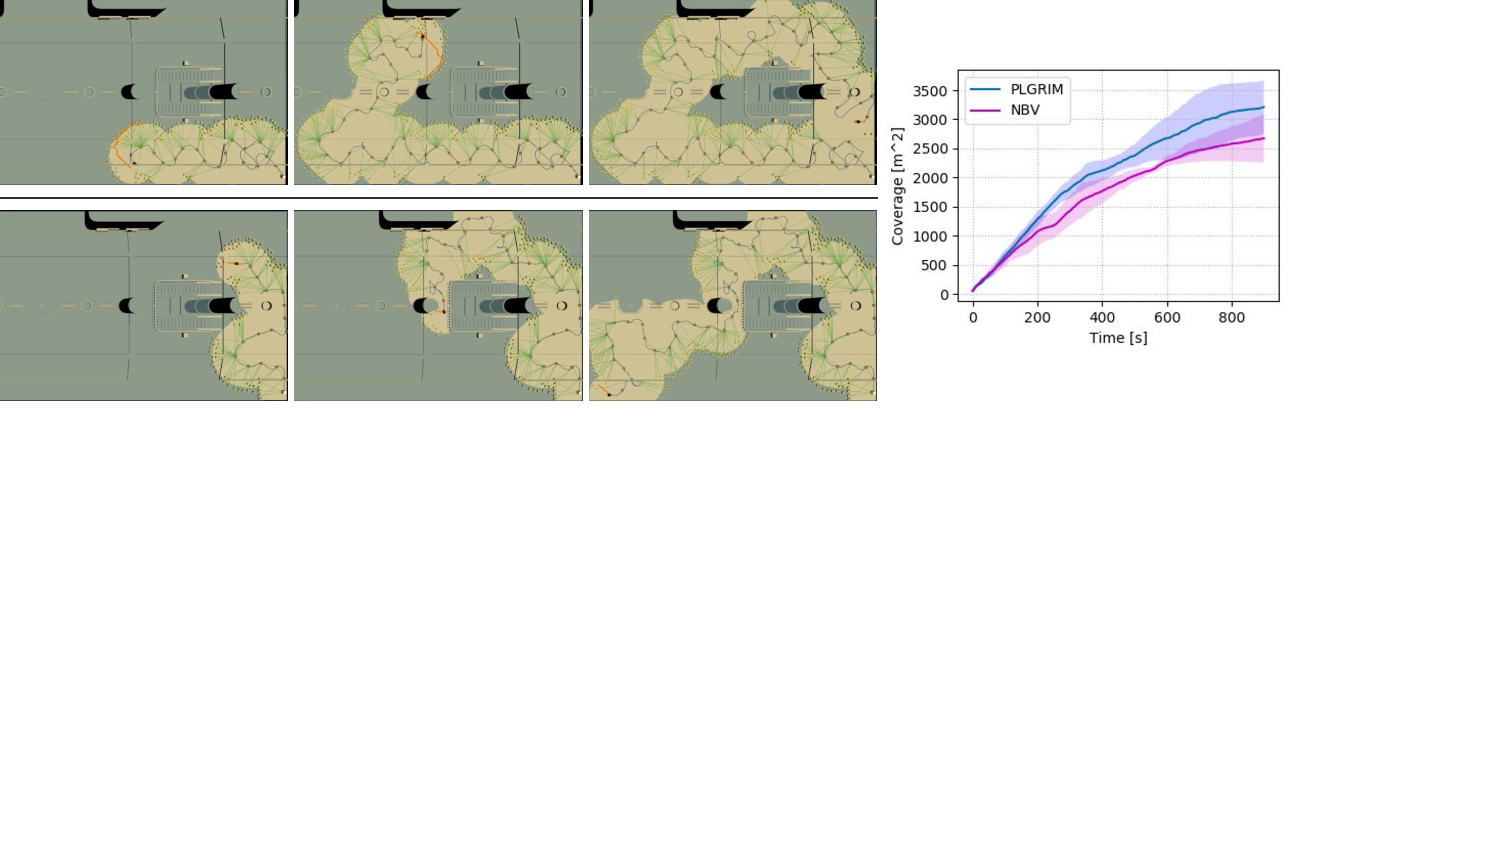
\includegraphics[width=1.\textwidth,trim={0 7.5cm 3cm 0},clip]{figures/s2_comparison.pdf}
  \caption{PLGRIM (top, across) vs. NBV (bottom, across). From left to right, the progress of coverage at $t=30$s, $t=50$s, and $t=80$s.  Note that PLGRIM explores more compactly and efficiently than the NBV approach.}
  \label{fig:station-baseline}
\end{figure}


In Fig.~\ref{fig:may-demo-plot}, shows the quantitative results during the autonomous exploration mission.
% (More experimental results will come.)

% \begin{figure}[!t]
%   \centering
%   \subfloat[Hardware Testing]{%
%     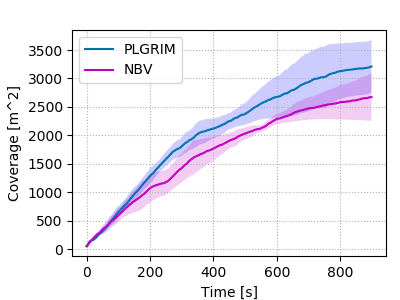
\includegraphics[width=.45\textwidth]{figures/subway_station_coverage.png}
%   }
%   \caption{Total distance traveled (blue), total area covered (purple), and the number of sectors on the environment (red) versus  time.}
%   \label{fig:may-demo-plot}
% \end{figure}


\subsection{Hardware Results}



% Coverage at time t
% : 4m FOV, following the robot traj, compute the total sweeping area

% Local IRM sweeping at time 0:t
% : 20m FOV, following the robot traj, compute the total reachable sweeping area

% relative coverage = Area(C) / Area(L)



%%%%%%%%%%%%%%%%%%%%%%%%%%%%%%%%%%%%%%%%%%%%%%%%%%%%%%%%%%%%%%%%%%%%%%%%%%%%%%%%
\section{Conclusion}\label{sec:conclusion}

In this work, we have developed a hierarchical framework for exploring large-scale unknown environments in a POMDP setting. 
To obtain a tractable solution we discretize the belief space into a robot and task-relevant graph structure which reduces our search space for good policies.
The hierarchical planning framework and formalization of the unified optimal policy enabled scaling up the highly complex coverage problems.
We demonstrate these capabilities in the high-fidelity dynamic simulation environment.  

The future work includes learning-based methods for graph expansion information gain estimation, and a richer incorporation of risk and time into the graph planning framework.
Another interesting venue is the extension of this framework to the multi-robot coverage problems.


\clearpage{}

\bibliography{references}  % .bib

\end{document}
